\item A position control system is to be designed such that maximum peak overshoot is less than 25 \%.
Further, appropriate error constant should be 50. For the motor to be used, load and torque
speed curve is shown below, where, J1 = 2 kg-m2
, J2 = 18 kg-m2
, f1 = 2 N-m-s/rad, f2 = 36 N-ms/rad. (Although obvious, consider position as the controlled variable and armature voltage as
the manipulated variable.). 
\begin{enumerate}[label=(\roman*)]
\item Design a lead compensator for the system.
\item Design a lag compensator for the system.
\end{enumerate}

\begin{figure}[!ht]
\centering
    \includegraphics[width=\columnwidth]{./figs/ee18btech11001/ee18btech11001_1.eps}
  \caption{}
  \label{fig:ee18btech11001_fig1}
\end{figure}
%
\solution
Solving the system shown in \ref{fig:ee18btech11001_fig1},

From load-torque curve of DC Motor
\begin{align}
   T_{m} &=  2V_{a} - \frac{2}{3}\omega_{1}
    \label{eq:ee18btech11001_1}
\end{align}
Let $T_{1}$ , $\omega_{1}$,$\theta_1{}$  be the Torque, Angular velocity, Angular displacement on $J_{1}$
\begin{align}
    T_{m} &= T_{1} + J_{1}\Ddot{\theta_{1}} + f_{1}\Dot{\theta_{1}} 
    \label{eq:ee18btech11001_2}
\end{align}
Similarly for $J_{2}$
\begin{align}
    T_{1} &=  J_{2}\Ddot{\theta_{2}} + f_{2}\Dot{\theta_{2}} 
    \label{eq:ee18btech11001_3}
    \\
    T_{2} &= \frac{N_{2}}{N_{1}} T_{1} \label{eq:ee18btech11001_4}
    \\
    \theta_{2} &= \frac{N_{1}}{N_{2}} \theta_{1} \label{eq:ee18btech11001_5}
\end{align}
    


On solving the equations \eqref{eq:ee18btech11001_1} , \eqref{eq:ee18btech11001_2}, \eqref{eq:ee18btech11001_3}, \eqref{eq:ee18btech11001_4} $\And$ \eqref{eq:ee18btech11001_5}

\begin{align}
    V_{a} &= 6\Ddot{\theta_{2}} + 10\Dot{\theta_{2}} \label{eq:ee18btech11001_6}
\end{align}

Taking Laplace transform
\begin{align}
   G(s) &=  K \frac{\theta (s)}{V_{a}(s)} = \frac{1}{2s(3s+5)} \label{eq:ee18btech11001_7}
\end{align}

From Error Constant  K = 500
\begin{align}
   G(s) &=  \frac{\theta (s)}{V_{a}(s)} = 250 \frac{1}{s(3s+5)} \label{eq:ee18btech11001_8}
   \\
   \zeta &= 0.0695
   \\
   M_{p} &= e^{\dfrac{-\zeta\pi}{\sqrt{1-\zeta^{2}}}} = 81.6\%
   \\
   Phase Margin &= \phi_{M} = \tan^{-1}(\dfrac{2\zeta}{\sqrt{-2\zeta^2 + \sqrt{4\zeta^4 + 1}}})
\end{align}

\begin{table}[!ht]
\centering
\item A position control system is to be designed such that maximum peak overshoot is less than 25 \%.
Further, appropriate error constant should be 50. For the motor to be used, load and torque
speed curve is shown below, where, J1 = 2 kg-m2
, J2 = 18 kg-m2
, f1 = 2 N-m-s/rad, f2 = 36 N-ms/rad. (Although obvious, consider position as the controlled variable and armature voltage as
the manipulated variable.). 
\begin{enumerate}[label=(\roman*)]
\item Design a lead compensator for the system.
\item Design a lag compensator for the system.
\end{enumerate}

\begin{figure}[!ht]
\centering
    \includegraphics[width=\columnwidth]{./figs/ee18btech11001/ee18btech11001_1.eps}
  \caption{}
  \label{fig:ee18btech11001_fig1}
\end{figure}
%
\solution
Solving the system shown in \ref{fig:ee18btech11001_fig1},

From load-torque curve of DC Motor
\begin{align}
   T_{m} &=  2V_{a} - \frac{2}{3}\omega_{1}
    \label{eq:ee18btech11001_1}
\end{align}
Let $T_{1}$ , $\omega_{1}$,$\theta_1{}$  be the Torque, Angular velocity, Angular displacement on $J_{1}$
\begin{align}
    T_{m} &= T_{1} + J_{1}\Ddot{\theta_{1}} + f_{1}\Dot{\theta_{1}} 
    \label{eq:ee18btech11001_2}
\end{align}
Similarly for $J_{2}$
\begin{align}
    T_{1} &=  J_{2}\Ddot{\theta_{2}} + f_{2}\Dot{\theta_{2}} 
    \label{eq:ee18btech11001_3}
    \\
    T_{2} &= \frac{N_{2}}{N_{1}} T_{1} \label{eq:ee18btech11001_4}
    \\
    \theta_{2} &= \frac{N_{1}}{N_{2}} \theta_{1} \label{eq:ee18btech11001_5}
\end{align}
    


On solving the equations \eqref{eq:ee18btech11001_1} , \eqref{eq:ee18btech11001_2}, \eqref{eq:ee18btech11001_3}, \eqref{eq:ee18btech11001_4} $\And$ \eqref{eq:ee18btech11001_5}

\begin{align}
    V_{a} &= 6\Ddot{\theta_{2}} + 10\Dot{\theta_{2}} \label{eq:ee18btech11001_6}
\end{align}

Taking Laplace transform
\begin{align}
   G(s) &=  K \frac{\theta (s)}{V_{a}(s)} = \frac{1}{2s(3s+5)} \label{eq:ee18btech11001_7}
\end{align}

From Error Constant  K = 500
\begin{align}
   G(s) &=  \frac{\theta (s)}{V_{a}(s)} = 250 \frac{1}{s(3s+5)} \label{eq:ee18btech11001_8}
   \\
   \zeta &= 0.0695
   \\
   M_{p} &= e^{\dfrac{-\zeta\pi}{\sqrt{1-\zeta^{2}}}} = 81.6\%
   \\
   Phase Margin &= \phi_{M} = \tan^{-1}(\dfrac{2\zeta}{\sqrt{-2\zeta^2 + \sqrt{4\zeta^4 + 1}}})
\end{align}

\begin{table}[!ht]
\centering
\item A position control system is to be designed such that maximum peak overshoot is less than 25 \%.
Further, appropriate error constant should be 50. For the motor to be used, load and torque
speed curve is shown below, where, J1 = 2 kg-m2
, J2 = 18 kg-m2
, f1 = 2 N-m-s/rad, f2 = 36 N-ms/rad. (Although obvious, consider position as the controlled variable and armature voltage as
the manipulated variable.). 
\begin{enumerate}[label=(\roman*)]
\item Design a lead compensator for the system.
\item Design a lag compensator for the system.
\end{enumerate}

\begin{figure}[!ht]
\centering
    \includegraphics[width=\columnwidth]{./figs/ee18btech11001/ee18btech11001_1.eps}
  \caption{}
  \label{fig:ee18btech11001_fig1}
\end{figure}
%
\solution
Solving the system shown in \ref{fig:ee18btech11001_fig1},

From load-torque curve of DC Motor
\begin{align}
   T_{m} &=  2V_{a} - \frac{2}{3}\omega_{1}
    \label{eq:ee18btech11001_1}
\end{align}
Let $T_{1}$ , $\omega_{1}$,$\theta_1{}$  be the Torque, Angular velocity, Angular displacement on $J_{1}$
\begin{align}
    T_{m} &= T_{1} + J_{1}\Ddot{\theta_{1}} + f_{1}\Dot{\theta_{1}} 
    \label{eq:ee18btech11001_2}
\end{align}
Similarly for $J_{2}$
\begin{align}
    T_{1} &=  J_{2}\Ddot{\theta_{2}} + f_{2}\Dot{\theta_{2}} 
    \label{eq:ee18btech11001_3}
    \\
    T_{2} &= \frac{N_{2}}{N_{1}} T_{1} \label{eq:ee18btech11001_4}
    \\
    \theta_{2} &= \frac{N_{1}}{N_{2}} \theta_{1} \label{eq:ee18btech11001_5}
\end{align}
    


On solving the equations \eqref{eq:ee18btech11001_1} , \eqref{eq:ee18btech11001_2}, \eqref{eq:ee18btech11001_3}, \eqref{eq:ee18btech11001_4} $\And$ \eqref{eq:ee18btech11001_5}

\begin{align}
    V_{a} &= 6\Ddot{\theta_{2}} + 10\Dot{\theta_{2}} \label{eq:ee18btech11001_6}
\end{align}

Taking Laplace transform
\begin{align}
   G(s) &=  K \frac{\theta (s)}{V_{a}(s)} = \frac{1}{2s(3s+5)} \label{eq:ee18btech11001_7}
\end{align}

From Error Constant  K = 500
\begin{align}
   G(s) &=  \frac{\theta (s)}{V_{a}(s)} = 250 \frac{1}{s(3s+5)} \label{eq:ee18btech11001_8}
   \\
   \zeta &= 0.0695
   \\
   M_{p} &= e^{\dfrac{-\zeta\pi}{\sqrt{1-\zeta^{2}}}} = 81.6\%
   \\
   Phase Margin &= \phi_{M} = \tan^{-1}(\dfrac{2\zeta}{\sqrt{-2\zeta^2 + \sqrt{4\zeta^4 + 1}}})
\end{align}

\begin{table}[!ht]
\centering
\item A position control system is to be designed such that maximum peak overshoot is less than 25 \%.
Further, appropriate error constant should be 50. For the motor to be used, load and torque
speed curve is shown below, where, J1 = 2 kg-m2
, J2 = 18 kg-m2
, f1 = 2 N-m-s/rad, f2 = 36 N-ms/rad. (Although obvious, consider position as the controlled variable and armature voltage as
the manipulated variable.). 
\begin{enumerate}[label=(\roman*)]
\item Design a lead compensator for the system.
\item Design a lag compensator for the system.
\end{enumerate}

\begin{figure}[!ht]
\centering
    \includegraphics[width=\columnwidth]{./figs/ee18btech11001/ee18btech11001_1.eps}
  \caption{}
  \label{fig:ee18btech11001_fig1}
\end{figure}
%
\solution
Solving the system shown in \ref{fig:ee18btech11001_fig1},

From load-torque curve of DC Motor
\begin{align}
   T_{m} &=  2V_{a} - \frac{2}{3}\omega_{1}
    \label{eq:ee18btech11001_1}
\end{align}
Let $T_{1}$ , $\omega_{1}$,$\theta_1{}$  be the Torque, Angular velocity, Angular displacement on $J_{1}$
\begin{align}
    T_{m} &= T_{1} + J_{1}\Ddot{\theta_{1}} + f_{1}\Dot{\theta_{1}} 
    \label{eq:ee18btech11001_2}
\end{align}
Similarly for $J_{2}$
\begin{align}
    T_{1} &=  J_{2}\Ddot{\theta_{2}} + f_{2}\Dot{\theta_{2}} 
    \label{eq:ee18btech11001_3}
    \\
    T_{2} &= \frac{N_{2}}{N_{1}} T_{1} \label{eq:ee18btech11001_4}
    \\
    \theta_{2} &= \frac{N_{1}}{N_{2}} \theta_{1} \label{eq:ee18btech11001_5}
\end{align}
    


On solving the equations \eqref{eq:ee18btech11001_1} , \eqref{eq:ee18btech11001_2}, \eqref{eq:ee18btech11001_3}, \eqref{eq:ee18btech11001_4} $\And$ \eqref{eq:ee18btech11001_5}

\begin{align}
    V_{a} &= 6\Ddot{\theta_{2}} + 10\Dot{\theta_{2}} \label{eq:ee18btech11001_6}
\end{align}

Taking Laplace transform
\begin{align}
   G(s) &=  K \frac{\theta (s)}{V_{a}(s)} = \frac{1}{2s(3s+5)} \label{eq:ee18btech11001_7}
\end{align}

From Error Constant  K = 500
\begin{align}
   G(s) &=  \frac{\theta (s)}{V_{a}(s)} = 250 \frac{1}{s(3s+5)} \label{eq:ee18btech11001_8}
   \\
   \zeta &= 0.0695
   \\
   M_{p} &= e^{\dfrac{-\zeta\pi}{\sqrt{1-\zeta^{2}}}} = 81.6\%
   \\
   Phase Margin &= \phi_{M} = \tan^{-1}(\dfrac{2\zeta}{\sqrt{-2\zeta^2 + \sqrt{4\zeta^4 + 1}}})
\end{align}

\begin{table}[!ht]
\centering
\input{./Tables/ee18btech11001.tex}
\caption{Table of Specifications}
\label{table:ee18btech11001}
\end{table}

$\phi_{max} = 39.5\degree-7.35\degree+$ correction factor

$\phi_{max} = 57\degree$

Designing a lead compensator
Let 
\begin{align}
   G_{c}(s) &=  \frac{1}{a}\frac{s + \frac{1}{T}}{s + \frac{1}{aT}} (a<1) \label{eq:ee18btech11001_9}
   \\
   \sin\phi_{max} &= \dfrac{a-1}{a+1}
   \\
   a &= 0.1
   \\
   |G(j\omega_{c})| &= \frac{1}{\sqrt{a}} = 10 dB
\end{align}
$\omega_{c} = 5\degree$ Refer \ref{fig:ee18btech11001_fig3}
\begin{align}
   T &= \frac{1}{\omega_{c}\sqrt{a}}
   \\
   T &= 0.632
   \\
   G_{c}(s) &=  10 \frac{s + 1.6}{s + 16}
   \\
   G(s)G_{c}(s)  &= 2500 \dfrac{s+1.6}{s(3s+5)(s+16)} \label{eq:ee18btech11001_10}
\end{align}

Designing a lag compensator
\begin{align}
   G_{c}(s) &=  \frac{1}{b}\frac{s + \frac{1}{T}}{s + \frac{1}{bT}} (b>1)  \label{eq:ee18btech11001_11}
   \\
   \phi_{max}  &= 39.5\degree -7.35\degree + correction factor
   \\
   \phi_{max} &= 45 \degree
\end{align}
\begin{figure}[!ht]
\centering
    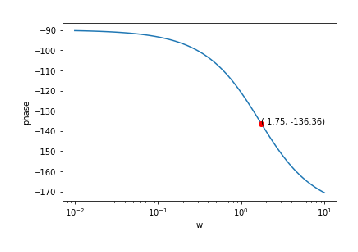
\includegraphics[width=\columnwidth]{./figs/ee18btech11001/ee18btech11001_3.eps}
  \caption{Phase plot of G(s)}
  \label{fig:ee18btech11001_fig2}
\end{figure}

$\omega_{c} = $ Frequency at which phase of bode plot of G(s) is -180 $+ \phi_{max}$ i.e. -135 \degree

$\omega_{c}  = 1.75 rad/sec$  as in Figure \ref{fig:ee18btech11001_fig2}

We place the zero at 
\begin{align} 
   \omega &= 0.2\omega_{c} = 0.35 rad/sec 
   \\
   \frac{1}{T} &= 0.35
   \\
   T &= 2.85
\end{align}
\begin{figure}[!ht]
\centering
    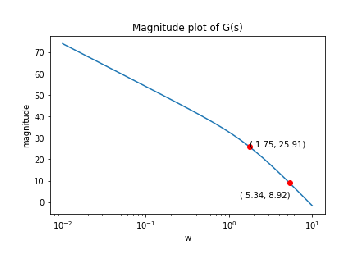
\includegraphics[width=\columnwidth]{./figs/ee18btech11001/ee18btech11001_2.eps}
  \caption{Magnitude plot of G(s)}
  \label{fig:ee18btech11001_fig3}
\end{figure}
The following code plots the following bode plots
\begin{lstlisting}
    codes/ee18btech11001/ee18btech11001_1.py
\end{lstlisting}

The magnitude of $G(j\omega)$ at the new gain crossover frequency  $\omega_{c} = 1.75 rad/sec$ is 26 dB as in figure \ref{fig:ee18btech11001_fig3}.In order to have $\omega_{c}$  as the new gain crossover frequency, the lag compensator
must give an attenuation of -26db at $\omega_{c}$
\begin{align}
    -20 \log{b} &= -26dB
    \\
    b &= 19.95 \approx 20
    \\
    G_{c}(s) &=  0.05\frac{s + 0.35}{s + 0.0175}
    \\
    G(s)G_{c}(s) &= 12.5 \dfrac{s+0.35}{s(3s+5)(s+0.0175)} \label{eq:ee18btech11001_12}
\end{align}
\text{Performance Evaluation of compensators}

\text{The following code plots the performance curves}

\begin{lstlisting}
    codes/ee18btech11001/ee18btech11001_2.py
\end{lstlisting}

\begin{figure}[!ht]
\centering
    \includegraphics[width=\columnwidth]{./figs/ee18btech11001/ee18btech11001_4.eps}
  \caption{Performance of Lead Compensator}
  \label{fig:ee18btech11001_fig4}
\end{figure}


\begin{figure}[!ht]
\centering
    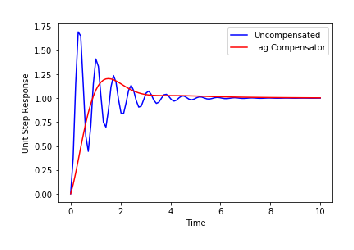
\includegraphics[width=\columnwidth]{./figs/ee18btech11001/ee18btech11001_5.eps}
  \caption{Performance of Lag Compensator}
  \label{fig:ee18btech11001_fig5}
\end{figure}






\begin{table}[!ht]
\centering
\input{./Tables/ee18btech11001_2.tex}
\caption{Performance comparison}
\label{table:ee18btech11001_2}
\end{table}


%\end{enumerate}
\caption{Table of Specifications}
\label{table:ee18btech11001}
\end{table}

$\phi_{max} = 39.5\degree-7.35\degree+$ correction factor

$\phi_{max} = 57\degree$

Designing a lead compensator
Let 
\begin{align}
   G_{c}(s) &=  \frac{1}{a}\frac{s + \frac{1}{T}}{s + \frac{1}{aT}} (a<1) \label{eq:ee18btech11001_9}
   \\
   \sin\phi_{max} &= \dfrac{a-1}{a+1}
   \\
   a &= 0.1
   \\
   |G(j\omega_{c})| &= \frac{1}{\sqrt{a}} = 10 dB
\end{align}
$\omega_{c} = 5\degree$ Refer \ref{fig:ee18btech11001_fig3}
\begin{align}
   T &= \frac{1}{\omega_{c}\sqrt{a}}
   \\
   T &= 0.632
   \\
   G_{c}(s) &=  10 \frac{s + 1.6}{s + 16}
   \\
   G(s)G_{c}(s)  &= 2500 \dfrac{s+1.6}{s(3s+5)(s+16)} \label{eq:ee18btech11001_10}
\end{align}

Designing a lag compensator
\begin{align}
   G_{c}(s) &=  \frac{1}{b}\frac{s + \frac{1}{T}}{s + \frac{1}{bT}} (b>1)  \label{eq:ee18btech11001_11}
   \\
   \phi_{max}  &= 39.5\degree -7.35\degree + correction factor
   \\
   \phi_{max} &= 45 \degree
\end{align}
\begin{figure}[!ht]
\centering
    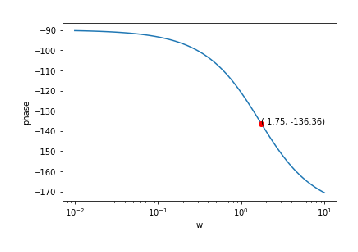
\includegraphics[width=\columnwidth]{./figs/ee18btech11001/ee18btech11001_3.eps}
  \caption{Phase plot of G(s)}
  \label{fig:ee18btech11001_fig2}
\end{figure}

$\omega_{c} = $ Frequency at which phase of bode plot of G(s) is -180 $+ \phi_{max}$ i.e. -135 \degree

$\omega_{c}  = 1.75 rad/sec$  as in Figure \ref{fig:ee18btech11001_fig2}

We place the zero at 
\begin{align} 
   \omega &= 0.2\omega_{c} = 0.35 rad/sec 
   \\
   \frac{1}{T} &= 0.35
   \\
   T &= 2.85
\end{align}
\begin{figure}[!ht]
\centering
    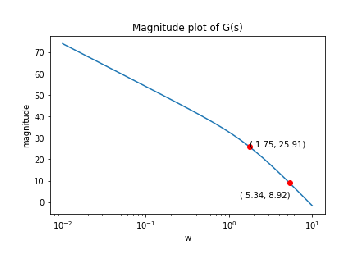
\includegraphics[width=\columnwidth]{./figs/ee18btech11001/ee18btech11001_2.eps}
  \caption{Magnitude plot of G(s)}
  \label{fig:ee18btech11001_fig3}
\end{figure}
The following code plots the following bode plots
\begin{lstlisting}
    codes/ee18btech11001/ee18btech11001_1.py
\end{lstlisting}

The magnitude of $G(j\omega)$ at the new gain crossover frequency  $\omega_{c} = 1.75 rad/sec$ is 26 dB as in figure \ref{fig:ee18btech11001_fig3}.In order to have $\omega_{c}$  as the new gain crossover frequency, the lag compensator
must give an attenuation of -26db at $\omega_{c}$
\begin{align}
    -20 \log{b} &= -26dB
    \\
    b &= 19.95 \approx 20
    \\
    G_{c}(s) &=  0.05\frac{s + 0.35}{s + 0.0175}
    \\
    G(s)G_{c}(s) &= 12.5 \dfrac{s+0.35}{s(3s+5)(s+0.0175)} \label{eq:ee18btech11001_12}
\end{align}
\text{Performance Evaluation of compensators}

\text{The following code plots the performance curves}

\begin{lstlisting}
    codes/ee18btech11001/ee18btech11001_2.py
\end{lstlisting}

\begin{figure}[!ht]
\centering
    \includegraphics[width=\columnwidth]{./figs/ee18btech11001/ee18btech11001_4.eps}
  \caption{Performance of Lead Compensator}
  \label{fig:ee18btech11001_fig4}
\end{figure}


\begin{figure}[!ht]
\centering
    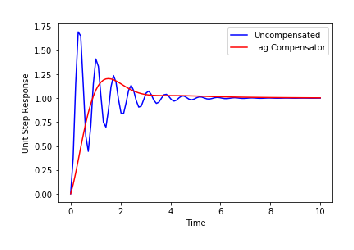
\includegraphics[width=\columnwidth]{./figs/ee18btech11001/ee18btech11001_5.eps}
  \caption{Performance of Lag Compensator}
  \label{fig:ee18btech11001_fig5}
\end{figure}






\begin{table}[!ht]
\centering
\input{./Tables/ee18btech11001_2.tex}
\caption{Performance comparison}
\label{table:ee18btech11001_2}
\end{table}


%\end{enumerate}
\caption{Table of Specifications}
\label{table:ee18btech11001}
\end{table}

$\phi_{max} = 39.5\degree-7.35\degree+$ correction factor

$\phi_{max} = 57\degree$

Designing a lead compensator
Let 
\begin{align}
   G_{c}(s) &=  \frac{1}{a}\frac{s + \frac{1}{T}}{s + \frac{1}{aT}} (a<1) \label{eq:ee18btech11001_9}
   \\
   \sin\phi_{max} &= \dfrac{a-1}{a+1}
   \\
   a &= 0.1
   \\
   |G(j\omega_{c})| &= \frac{1}{\sqrt{a}} = 10 dB
\end{align}
$\omega_{c} = 5\degree$ Refer \ref{fig:ee18btech11001_fig3}
\begin{align}
   T &= \frac{1}{\omega_{c}\sqrt{a}}
   \\
   T &= 0.632
   \\
   G_{c}(s) &=  10 \frac{s + 1.6}{s + 16}
   \\
   G(s)G_{c}(s)  &= 2500 \dfrac{s+1.6}{s(3s+5)(s+16)} \label{eq:ee18btech11001_10}
\end{align}

Designing a lag compensator
\begin{align}
   G_{c}(s) &=  \frac{1}{b}\frac{s + \frac{1}{T}}{s + \frac{1}{bT}} (b>1)  \label{eq:ee18btech11001_11}
   \\
   \phi_{max}  &= 39.5\degree -7.35\degree + correction factor
   \\
   \phi_{max} &= 45 \degree
\end{align}
\begin{figure}[!ht]
\centering
    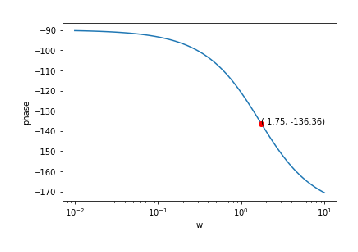
\includegraphics[width=\columnwidth]{./figs/ee18btech11001/ee18btech11001_3.eps}
  \caption{Phase plot of G(s)}
  \label{fig:ee18btech11001_fig2}
\end{figure}

$\omega_{c} = $ Frequency at which phase of bode plot of G(s) is -180 $+ \phi_{max}$ i.e. -135 \degree

$\omega_{c}  = 1.75 rad/sec$  as in Figure \ref{fig:ee18btech11001_fig2}

We place the zero at 
\begin{align} 
   \omega &= 0.2\omega_{c} = 0.35 rad/sec 
   \\
   \frac{1}{T} &= 0.35
   \\
   T &= 2.85
\end{align}
\begin{figure}[!ht]
\centering
    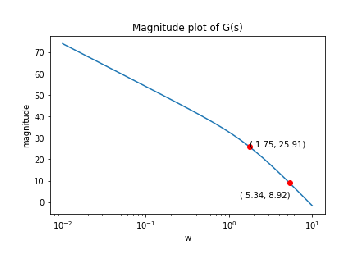
\includegraphics[width=\columnwidth]{./figs/ee18btech11001/ee18btech11001_2.eps}
  \caption{Magnitude plot of G(s)}
  \label{fig:ee18btech11001_fig3}
\end{figure}
The following code plots the following bode plots
\begin{lstlisting}
    codes/ee18btech11001/ee18btech11001_1.py
\end{lstlisting}

The magnitude of $G(j\omega)$ at the new gain crossover frequency  $\omega_{c} = 1.75 rad/sec$ is 26 dB as in figure \ref{fig:ee18btech11001_fig3}.In order to have $\omega_{c}$  as the new gain crossover frequency, the lag compensator
must give an attenuation of -26db at $\omega_{c}$
\begin{align}
    -20 \log{b} &= -26dB
    \\
    b &= 19.95 \approx 20
    \\
    G_{c}(s) &=  0.05\frac{s + 0.35}{s + 0.0175}
    \\
    G(s)G_{c}(s) &= 12.5 \dfrac{s+0.35}{s(3s+5)(s+0.0175)} \label{eq:ee18btech11001_12}
\end{align}
\text{Performance Evaluation of compensators}

\text{The following code plots the performance curves}

\begin{lstlisting}
    codes/ee18btech11001/ee18btech11001_2.py
\end{lstlisting}

\begin{figure}[!ht]
\centering
    \includegraphics[width=\columnwidth]{./figs/ee18btech11001/ee18btech11001_4.eps}
  \caption{Performance of Lead Compensator}
  \label{fig:ee18btech11001_fig4}
\end{figure}


\begin{figure}[!ht]
\centering
    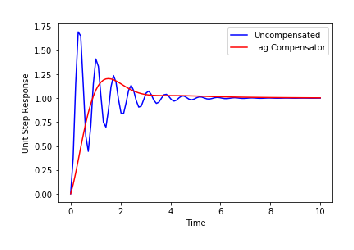
\includegraphics[width=\columnwidth]{./figs/ee18btech11001/ee18btech11001_5.eps}
  \caption{Performance of Lag Compensator}
  \label{fig:ee18btech11001_fig5}
\end{figure}






\begin{table}[!ht]
\centering
\input{./Tables/ee18btech11001_2.tex}
\caption{Performance comparison}
\label{table:ee18btech11001_2}
\end{table}


%\end{enumerate}
\caption{Table of Specifications}
\label{table:ee18btech11001}
\end{table}

$\phi_{max} = 39.5\degree-7.35\degree+$ correction factor

$\phi_{max} = 57\degree$

Designing a lead compensator
Let 
\begin{align}
   G_{c}(s) &=  \frac{1}{a}\frac{s + \frac{1}{T}}{s + \frac{1}{aT}} (a<1) \label{eq:ee18btech11001_9}
   \\
   \sin\phi_{max} &= \dfrac{a-1}{a+1}
   \\
   a &= 0.1
   \\
   |G(j\omega_{c})| &= \frac{1}{\sqrt{a}} = 10 dB
\end{align}
$\omega_{c} = 5\degree$ Refer \ref{fig:ee18btech11001_fig3}
\begin{align}
   T &= \frac{1}{\omega_{c}\sqrt{a}}
   \\
   T &= 0.632
   \\
   G_{c}(s) &=  10 \frac{s + 1.6}{s + 16}
   \\
   G(s)G_{c}(s)  &= 2500 \dfrac{s+1.6}{s(3s+5)(s+16)} \label{eq:ee18btech11001_10}
\end{align}

Designing a lag compensator
\begin{align}
   G_{c}(s) &=  \frac{1}{b}\frac{s + \frac{1}{T}}{s + \frac{1}{bT}} (b>1)  \label{eq:ee18btech11001_11}
   \\
   \phi_{max}  &= 39.5\degree -7.35\degree + correction factor
   \\
   \phi_{max} &= 45 \degree
\end{align}
\begin{figure}[!ht]
\centering
    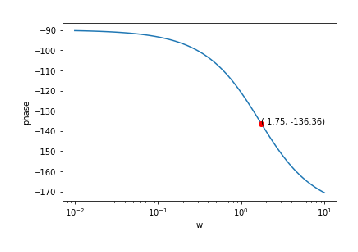
\includegraphics[width=\columnwidth]{./figs/ee18btech11001/ee18btech11001_3.eps}
  \caption{Phase plot of G(s)}
  \label{fig:ee18btech11001_fig2}
\end{figure}

$\omega_{c} = $ Frequency at which phase of bode plot of G(s) is -180 $+ \phi_{max}$ i.e. -135 \degree

$\omega_{c}  = 1.75 rad/sec$  as in Figure \ref{fig:ee18btech11001_fig2}

We place the zero at 
\begin{align} 
   \omega &= 0.2\omega_{c} = 0.35 rad/sec 
   \\
   \frac{1}{T} &= 0.35
   \\
   T &= 2.85
\end{align}
\begin{figure}[!ht]
\centering
    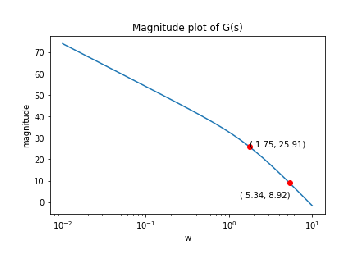
\includegraphics[width=\columnwidth]{./figs/ee18btech11001/ee18btech11001_2.eps}
  \caption{Magnitude plot of G(s)}
  \label{fig:ee18btech11001_fig3}
\end{figure}
The following code plots the following bode plots
\begin{lstlisting}
    codes/ee18btech11001/ee18btech11001_1.py
\end{lstlisting}

The magnitude of $G(j\omega)$ at the new gain crossover frequency  $\omega_{c} = 1.75 rad/sec$ is 26 dB as in figure \ref{fig:ee18btech11001_fig3}.In order to have $\omega_{c}$  as the new gain crossover frequency, the lag compensator
must give an attenuation of -26db at $\omega_{c}$
\begin{align}
    -20 \log{b} &= -26dB
    \\
    b &= 19.95 \approx 20
    \\
    G_{c}(s) &=  0.05\frac{s + 0.35}{s + 0.0175}
    \\
    G(s)G_{c}(s) &= 12.5 \dfrac{s+0.35}{s(3s+5)(s+0.0175)} \label{eq:ee18btech11001_12}
\end{align}
\text{Performance Evaluation of compensators}

\text{The following code plots the performance curves}

\begin{lstlisting}
    codes/ee18btech11001/ee18btech11001_2.py
\end{lstlisting}

\begin{figure}[!ht]
\centering
    \includegraphics[width=\columnwidth]{./figs/ee18btech11001/ee18btech11001_4.eps}
  \caption{Performance of Lead Compensator}
  \label{fig:ee18btech11001_fig4}
\end{figure}


\begin{figure}[!ht]
\centering
    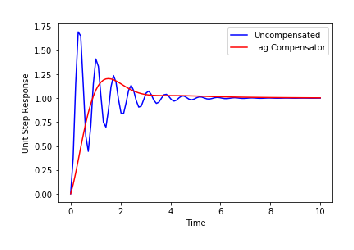
\includegraphics[width=\columnwidth]{./figs/ee18btech11001/ee18btech11001_5.eps}
  \caption{Performance of Lag Compensator}
  \label{fig:ee18btech11001_fig5}
\end{figure}






\begin{table}[!ht]
\centering
\input{./Tables/ee18btech11001_2.tex}
\caption{Performance comparison}
\label{table:ee18btech11001_2}
\end{table}


%\end{enumerate}